\documentclass[../main.tex]{subfiles}

\begin{document}

\section{Esempi}
Iniziamo a vedere qualche esempio di approssimazione di funzione su dati generati casualmente.
Gli esempi sono presi dal \href{https://github.com/cMancio00/B-Spline/blob/main/esempi.ipynb}{Notebook Jupyter} della repository.
Mostriamo inizialmente l'esempio più semplice, ovvero l'approssimazione della retta in figura \ref*{fig:retta}. Cominciamo importando 
le librerie necessarie e creando una base B-Spline e una base gerarchica.

\begin{lstlisting}[language=Python, caption={Dichiarazione della base}]

from Curve_Fitting import Model
from HB_Spline import HB_Spline
from B_Spline import B_Spline
import numpy as np
from matplotlib import pyplot as plt

np.random.seed(1304)

base  = B_Spline(
        knots=np.linspace(0,10,5+1),
        order=3
    )

hb = HB_Spline(base)

\end{lstlisting}

Nell'esempio è stata creata una base di ordine 3 con nodi uniformi. Il dominio dei nodi può essere arbitrario. In tutti gli esempi verrà 
fatto coincidere con il dominio dei dati solo per comodità nella rifinitura.
Passiamo ora alla generazione dei dati. Per scopi di riproducibilità è stato impostato un seme. Per evitare problemi di dimensionalità 
il numero di dati equivale al numero di elementi nel vettore delle \textbf{ascisse di valutazione}. Un altro metodo potrebbe essere 
quello di scegliere in maniera equiprobabile dei dati da quelli generati. 

\begin{lstlisting}[language=Python, caption={Creazione e fit del modello}]
samples = np.shape(
    base.compute_base().get_collocation_matrix()
)[1]

x = np.linspace(0, 10, samples)
y= x + np.random.normal(0, 1, samples)

data = np.matrix([x, y]).T
\end{lstlisting} 

A questo punto possiamo creare il modello passando la base gerarchica(che non essendo rifinita equivale alla B-Spline madre) e i dati
che abbiamo generato.

\begin{lstlisting}[language=Python,caption={Plot dei risultati}]
model = Model(
    base=hb,
    data=data
).fit()

model.plot()
plt.plot(x, x, "y-", label="real")
plt.legend(loc="best")
\end{lstlisting}
Otteniamo l'output come mostrato in figura \ref{fig:retta_fit}
\begin{figure}
    \caption{Approssimazione di una retta}
    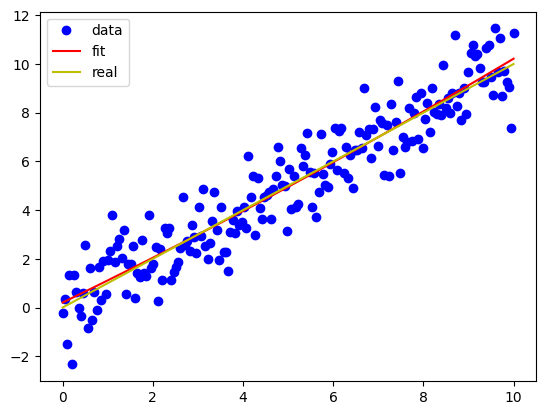
\includegraphics{Immagini/esempi/retta.png}
    \centering
    \label{fig:retta_fit}
\end{figure}
\end{document}